%!TEX program = xelatex
\documentclass[a4paper]{ctexart}

\usepackage{listings} 
\usepackage{geometry}
\usepackage{booktabs}
\usepackage{graphicx}
\usepackage{tabularx}
\usepackage{multirow}
\usepackage{enumitem}
\usepackage[bottom]{footmisc}

\renewcommand{\multirowsetup}{\centering}

\geometry{
    left=23mm,
    right=23mm,
    top=23mm,
    bottom=23mm,
}

\setlength{\parskip}{0.5em}

\title{CodeOcean 项目启动文档}
\author{
  曾少勋 171250603\\
  刘洪禹 171840773\\
  黄国钊 171250530\\
  夏雨笛 171250011\\
}
\date{\today}

\begin{document}

\maketitle

\begin{abstract}
  本项目为 CodeOcean 小组在 2020 年春季学期《需求与商业模式创新》课程中大作业设计的同名项目,此文档为其启动文档,记录了项目简介、商业模式画布要点及相关分析。
\end{abstract}

\tableofcontents

\newpage

\setlength{\parskip}{1em}


\section{项目简介}

CodeOcean 为一开源编程学习平台,主要由一下四大功能组成:网课教学、答案外卖、问答平台、文档中心。

网课教学,类似 MOOC,与企业、高校合作,提供优质课程,通过录播、直播、作业(OJ)、考试等方式,帮助用户学习掌握新知识。课程分为两种:一种是长期课程,全程往往在十几小时以上,帮助用户系统地了解一方面的知识;另一种课程则是短视频小课,长度在 5 分钟左右,帮助用户迅速学会一个小知识点,可以更合理地利用用户的碎片化时间。大部分课程都会提供免费试听的部分,其后内容需要收费。用户通过办理会员可以免费观看短视频小课,与此同时,通过使用本平台其他功能,也可以获得一定的积分,用于购买课程时抵现。

答案外卖,是本平台的核心创新功能之一,灵感来自外卖、嘀嘀打车等服务。提问者可以提出问题,支付一定的解答费,会有“解答小哥”接单并提供一对一解答。平台提供协作编程环境,可以使得提问者与“解答小哥”同时编辑代码,在问题解决后,提问者与“解答小哥”会进行双向评价,基于好评制度保证解答的质量。“解答小哥”会获得一定比例的解答费作为报酬,好评率高的还可以获得额外奖励。“解答小哥”主要由在校大学生组成,经过一定的资质认证即可上任,使得本平台成为一个可靠的兼职平台。在传统的问答平台,用户往往需要等待很久才会有答案,而且往往只会得到答案本身而非解决过程,正所谓“授人以鱼,不如授人以渔”,答案外卖服务使得用户即使获得答案并了解解答过程,更透彻地理解问题。

问答平台\footnote{CodeOcean 问答中心部分的功能灵感来源于本小组成员参加 2019 年华东 hackathon 时的一等奖获奖项目 BugStranding,项目地址:https://github.com/Hackathon2019EastChina/BugStranding-Naive}基于 docker 与在线版 vscode,提问者提问时,平台会自动生成 docker 环境,并在启用运行在线版 vscode,提问者将问题代码复制到此环境中复现问题,解答者打开网页即可修改并实时看到结果,免去解答者配置环境的过程,增加交流效率。解答者提交解答后,其修改内容会自动以 diff 的形式展现,使得后来者可以一目了然。这也是本平台的创新功能之一。相比之下,传统的问答平台需要用户手动复制代码,而提问者往往并不清楚代码的问题到底出现在哪里,常常会漏掉关键部分,使得回答者无从下手;其次,传统问答平台往往只要求提问者提交代码片段,回答者难以运行整个项目,只能对提问者提出一些修改建议,不断与提问者确认结果,十分耗时。

文档中心收集了各大项目官方文档,同时允许用户贡献,基于 wiki,使得所有人都可以自由编辑,文档中的代码可以在直接沙盒中运行,用户可以随时修改并观察结果。相较于传统的文档,直接执行代码省去了用户配置环境、切换窗口、复制粘贴的时间,保障了用户思维的连续性,增加了用户学习的效率。相较于博客,在文档中心,经典的算法、程序片段等同样的内容仅出现一次,并由用户不断完善,避免了用户在海量博文中进行寻找与甄别,节约了用户的时间。

\section{度量数值}

本文档共包含了 33 个要点与 27 条关联关系。平均要点数量约为4个。要点的联系详见第三部分,每个联系之前有要点位置的标注,例如1a表示关键业务的第a条要点。

\section{商业模式画布}

\subsection{要点概述}

\begin{center}
  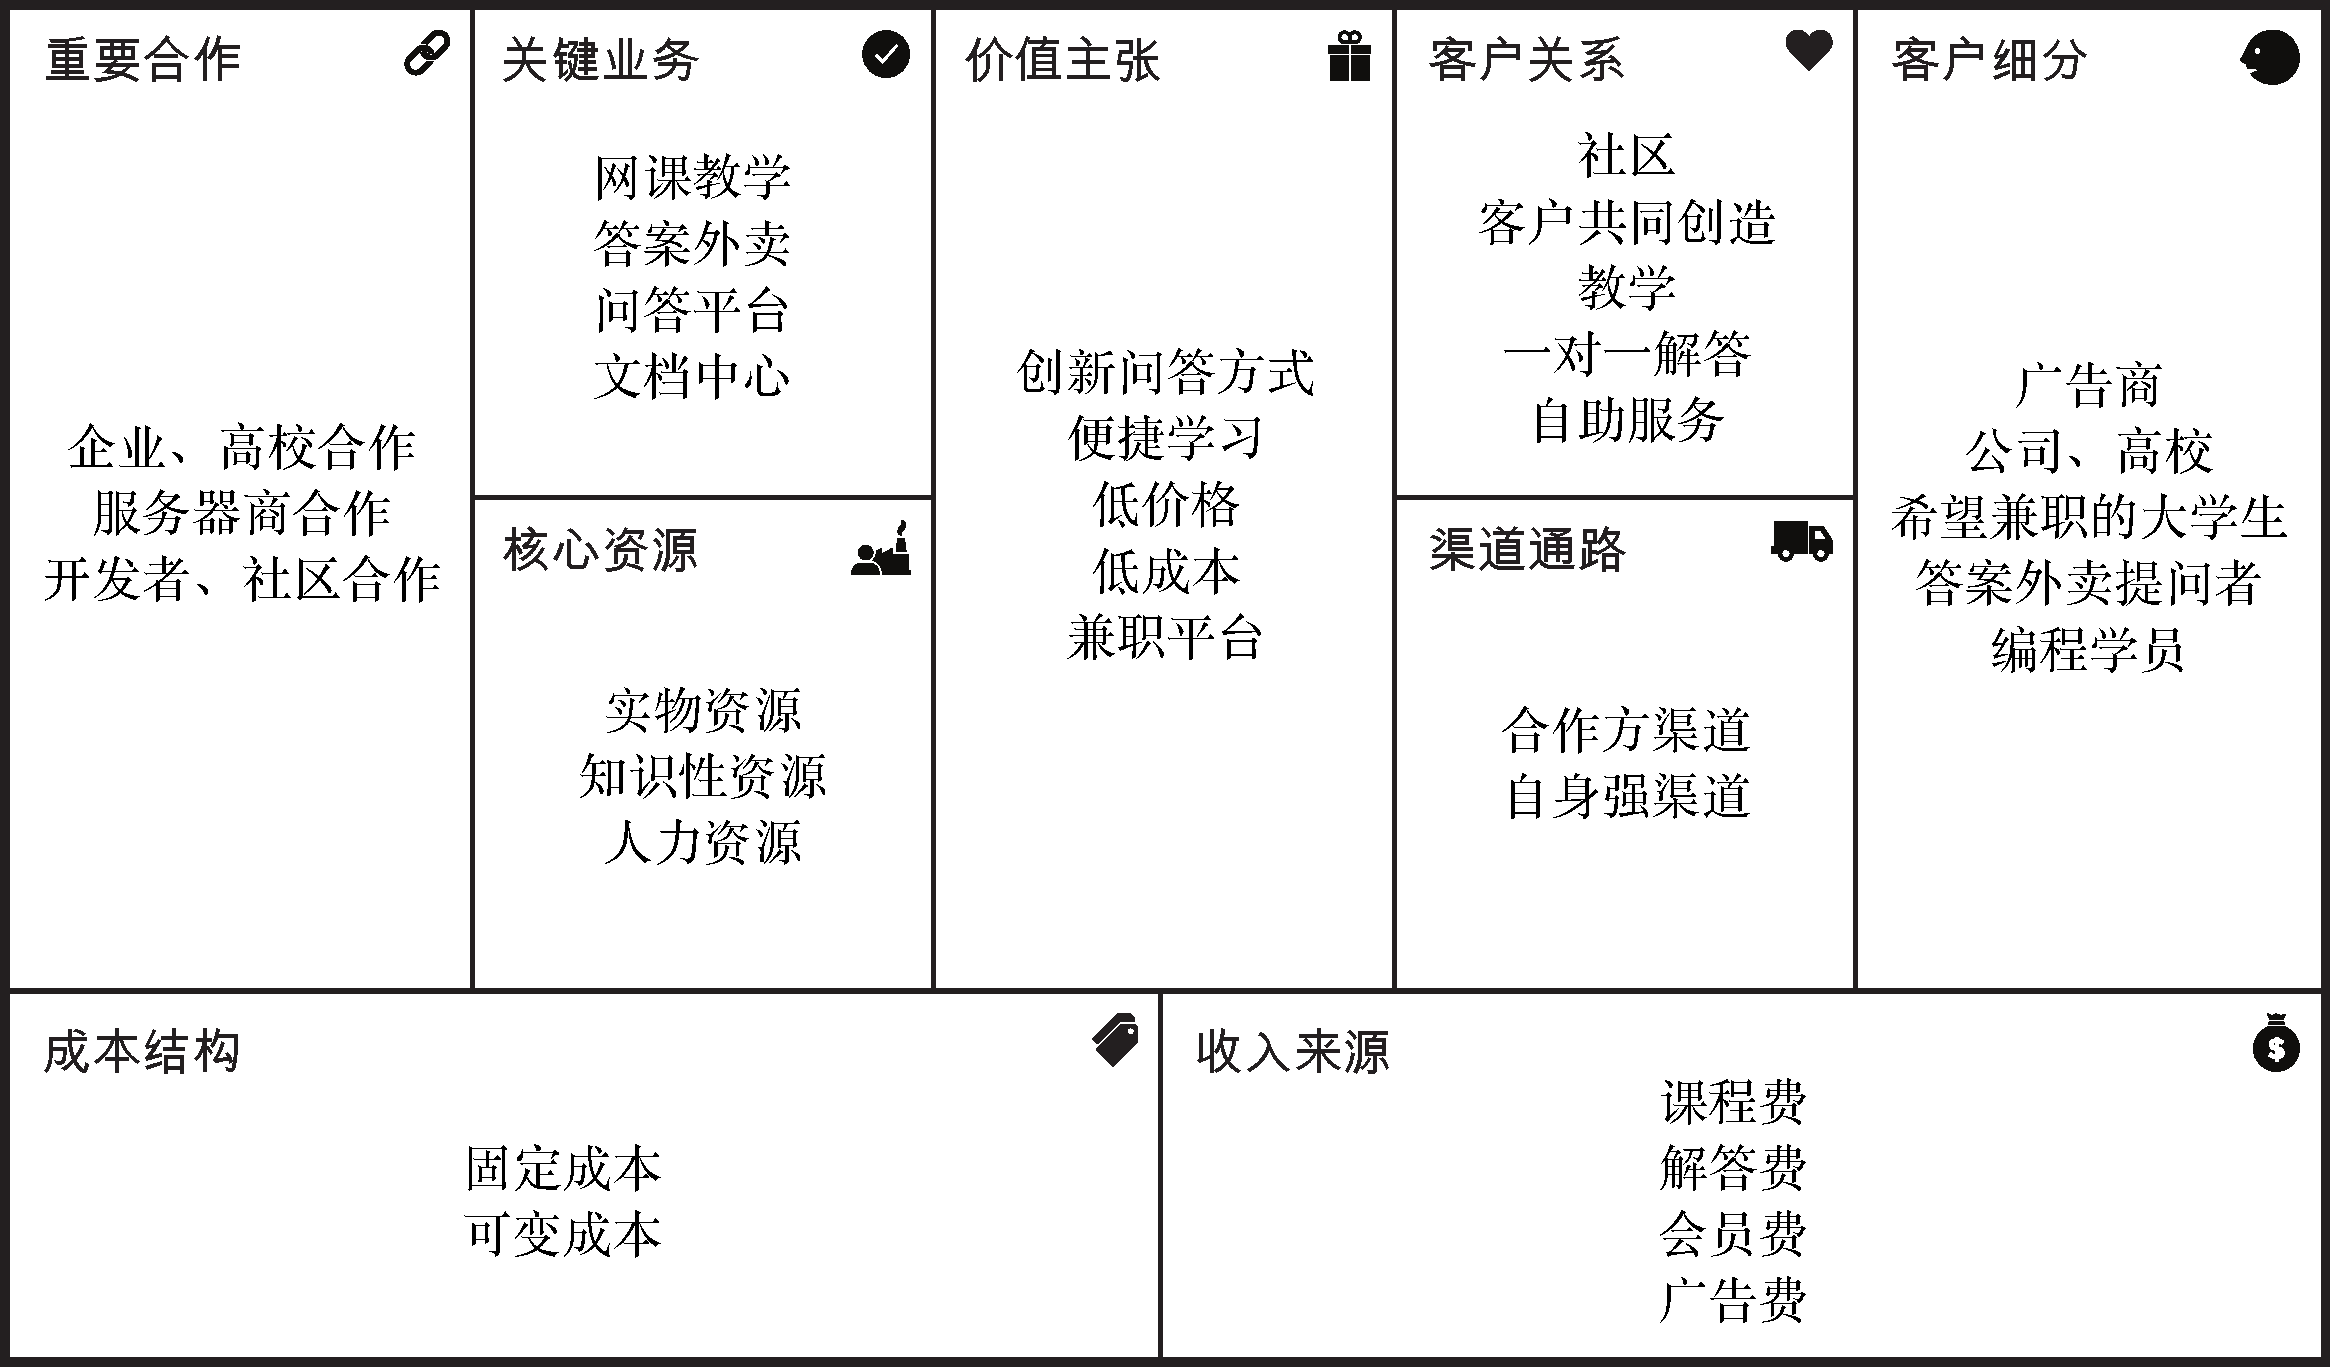
\includegraphics[width=16cm]{canvas}
\end{center}

\subsection{要点介绍}

\subsubsection{关键业务}

\begin{enumerate}[label=\alph*.]
  \item 网课教学:提供优质课程,通过录播、直播、作业(OJ)、考试等方式,帮助用户学习掌握新知识。课程有长期和短期两种,详见项目简介中的对应模块介绍。
  \item 答案外卖:提问者可以提出问题,支付一定的解答费,会有“解答小哥”接单并提供一对一解答。在问题解决后,提问者与“解答小哥”会进行双向评价,基于好评制度保证解答的质量。“解答小哥”会获得一定比例的解答费作为报酬,好评率高的还可以获得额外奖励。详见项目简介中的对应模块介绍。
  \item 问答平台:基于 docker 与在线版 vscode,提问者提问时,平台会自动生成 docker 环境,并在启用运行在线版 vscode,提问者将问题代码复制到此环境中复现问题,解答者打开网页即可修改并实时看到结果。解答者提交解答后,其修改内容会自动以 diff 的形式展现,使得后来者可以一目了然。详见项目简介中的对应模块介绍。
  \item 文档中心:收集了各大项目官方文档,同时允许用户贡献,基于 wiki,使得所有人都可以自由编辑,文档中的代码可以在直接沙盒中运行,用户可以随时修改并观察结果。详见项目简介中的对应模块介绍。
\end{enumerate}

\subsubsection{价值主张}

\begin{enumerate}[label=\alph*.]
  \item 创新问答方式:现有的问答平台,在用户提出问题后,往往需要经过较长时间的等待才能获得答案。本平台提供的答案外卖服务,尚未在市场出现,用户可以通过支付一定的费用,让获取答案像叫外卖、打车一样简单,是一次创新的尝试。
  \item 便捷学习:用户在问答中心提问时可以直接将代码放入 docker,回答者可以直接在网页版 vscode 中回答,无需配置环境。文档中心中的代码都可以直接在沙盒中执行,便于用户修改、查看结果,提升了学习效率。
  \item 低价格:增加宣传力度,增加用户数量,降低课程价格,以量取胜。
  \item 低成本:答案外卖使得用户花费少量金钱即可解决问题,节约了用户大量的时间,使得用户可以做更多有价值的事情。
  \item 兼职平台:用户达到一定资质便可注册为“解答小哥”,接取答案外卖订单,并获得一定报酬,为大学生等群体创造了一个可靠的兼职平台。
\end{enumerate}

\subsubsection{客户关系}

\begin{enumerate}[label=\alph*.]
  \item 社区:对某一问题感兴趣的用户群可以就这一问题进行讨论,发表自己独到的见解和解题思路,从而形成社区。
  \item 客户共同创造:任何用户都可以在问答平台上提问或解答,同时任何用户也可以贡献出自己对于一些经典算法解答的代码沙盒。人人都可以在平台上创造资源和使用资源,使平台的资源更加丰富。
  \item 教学:平台老师可以开设线上课程教学,其他对这一课程感兴趣的用户可以来听课。
  \item 一对一解答:用户可以通过答案外卖获得专属私人服务,一对一讲解为用户提供私人咨询。
  \item 自助服务:用户可以借助代码沙盒进行练习,自行搜索相关解答、提出问题,浏览文档。
\end{enumerate}

\subsubsection{重要合作}

\begin{enumerate}[label=\alph*.]
  \item 企业、高校合作:教学课程是平台关键业务的重要一环。与企业、高校合作,既能通过规模效应减少联系资深人士在平台上开设课程的平均成本,也能有效延长讲师在平台驻扎的年限。
  \item 服务器商合作:与服务器商合作,为其提供宣传,推荐用户在学习中使用,可以为其增加潜在用户,同时本平台也能优惠使用其服务。
  \item 开发者、社区合作:与各软件项目的开发者、开发社区合作,平台整理和收录其开发的项目的文档,开发者和社区可以通过 docker 部署一些简单的项目使用代码,帮助新手更快地上手其开发的工具,对于平台和项目的宣传都有促进作用,实现双赢。
\end{enumerate}

\subsubsection{收入来源}

\begin{enumerate}[label=\alph*.]
  \item 课程费:教师可以开设一些付费课程,可以是长期的大型课程,也可以是一些短视频小课,用户需要付费才能查看这些课程的内容,该网站为这些课程提供平台,相应地收取一些课程收入的抽成作为回报。
  \item 解答费:用户解答费用的抽成。用户可以通过付费可以对认证用户进行私下的问题咨询,类似地网站会抽取一定比例的费用作为提供平台的回报。
  \item 会员费:因为存在短期课程,网站开设会员制度,会员可以免除学习短期课程的费用,与教师的分成可以具体讨论。
  \item 广告费:网站提供一些区域作为发布广告的场所,从广告厂商处收取费用。
\end{enumerate}

\subsubsection{核心资源}

\begin{enumerate}[label=\alph*.]
  \item 实物资源:所拥有的实物资源主要是为了支持系统的在线平台,因此需要高性能的服务器,以满足大量用户的代码沙盒的使用需求。
  \item 知识性资源:主要由用户生产的资料组成。包括开设的课程、用户提出的问题以及回答、用户发布的文档,这些共同组成了平台的知识性资源。
  \item 人力资源:包括开发人员和核心的用户。平台的开发团队、招募或认证的师资队伍、解答问题的工程师队伍、出色的回答者都是重要的人力资源。
\end{enumerate}

\subsubsection{成本结构}

\begin{enumerate}[label=\alph*.]
  \item 固定成本:包括雇用开发人员的成本、维护物理服务器的成本、管理员工工资、机房用电、网络费用等。这些支出不论平台是否正常运行都需要支付,因此归为固定成本。
  \item 可变成本:包括雇用维护人员的成本、雇用客服人员的成本,此外,该系统需要有服务的提供者(课程的开设和问题的回答者),因此为了让平台有一些初始化的课程内容和认证工程师,还需要支付聘请公司、高校教师的合作费、平台的宣传推广费。这些支出是平台运行时决定的,因此归为可变成本。
\end{enumerate}

\subsubsection{渠道通路}

\begin{enumerate}[label=\alph*.]
  \item 合作方渠道:与企业、高校的合作与宣传,与已有项目的合作与宣传,可以迅速提升知名度。同时,高品质的企业、高校可以提供优质的课程,从而吸引用户付费学习,与此同时,企业、高校举办的直播、答疑等交流活动也可以进一步提升评价。
  \item 自身强渠道:平台吸引部分想获得额外收益的高水平人群,作为“解答小哥”一对一回答问题,通过评价制度保证服务质量,从而获得良好的口碑,进一步提升知名度。
\end{enumerate}

\subsubsection{客户细分}

\begin{enumerate}[label=\alph*.]
  \item 广告商:投放广告,增加流量。
  \item 公司、高校:开设课程,赚取课程费。
  \item 希望兼职的大学生:成为“解答小哥”,通过解答问题获取收益。
  \item 答案外卖提问者:通过答案外卖服务,支付解答费,获得一对一解答。
  \item 编程学员:参加课程、浏览文档、问答社区。
\end{enumerate}

\subsection{要点联系}

\paragraph{1a(网课教学), 4a(企业、高校合作)}由于要开设网课程,因此需要和高校或是企业合作,以此来获得优质的师资开设网上课程。
\paragraph{1a(网课教学), 5a(课程费)}平台提供付费课程,当用户购买课程后,平台可以从用户支付的课程费中抽取一定比例,作为平台收入的一部分。
\paragraph{1b(答案外卖), 2b(兼职平台)}“解答小哥”可以通过解答问题获取收益,使得本平台成为一个可靠的兼职平台。
\paragraph{1b(答案外卖), 5b(解答费)}在用户使用答案外卖服务的同时,平台会抽取解答费的一部分作为收入。
\paragraph{1c(问答平台), 2a(便捷学习)}基于 docker 的服务体现了便利性,用户之间的交流成本更低。
\paragraph{1d(文档中心), 4b(开发者、社区合作)}为了提供优质的文档,需要和大量的项目作者、社区进行合作。
\paragraph{2a(创新问答方式), 3d(一对一解答)}通过平台为用户提供了创新问答方式这一价值主张,提问者随时提问,业内高手一对一解答,创建了一个便捷提问的平台。
\paragraph{2b(兼职平台), 4a(企业、高校合作)}平台为一些高水平用户提供了额外的收入渠道,使得企业、高校更加愿意合作。
\paragraph{3b(客户共同创造), 6b(知识性资源)}本平台只是提供了一个用户自由问答、编写文档的地方,用户所实际受益的资源,大部分都来自其他用户的贡献,而这正是本平台的核心资源之一。
\paragraph{3c(教学), 4a(企业、高校合作)}希望接受相关知识教育的人群是潜在客户,与企业、高校的合作能在宣传和教育资源上帮助吸引目标群体。
\paragraph{4a(企业、高校合作), 6b(知识性资源)}与企业、高校的合作可以为本平台提供十分优质的课程资源,这是本平台的核心资源之一。
\paragraph{4a(企业、高校合作), 7a(可变成本)}与服务器厂商的合作能降低服务器成本。
\paragraph{4b(企业、高校合作), 7b(固定成本)}与企业、高校的长期合作能降低联系成本。
\paragraph{6a(实物资源), 7a(固定成本)}核心资源中的服务器等资产属于必须要支付的固定成本。
\paragraph{6c(人力资源), 7b(可变成本)}招募师资队伍、工程师队伍需要根据各人水平不同支付不同的薪水,属于可变成本。
\paragraph{2b(兼职平台), 5a(课程费), 5b(解答费)}平台主张提供便捷提问渠道的同时,抽成用户的解答费用产生收入。
\paragraph{4a(企业、高校合作), 5a(课程费), 5c(会员费)}与企业、高校形成合作关系能增加开设课程的数量,用户会有更多的课程可以选择,平台在课程上的收入会增加,也能吸收更多的会员,增加会员费收入。
\paragraph{4c(开发者、社区合作), 5b(解答费), 5d(广告费)}与项目开发者、社区合作,吸引用户,促进社区建设增加,促进使用答案外卖的人群数量增加,广告收益增加。
\paragraph{8a(合作方渠道), 9a(广告商), 9b(公司、高校)}众多的合作方渠道使得有许多利益相关方均可通过本平台获益,使得本平台客户多边化,受众广泛、来源稳定。
\paragraph{2a(便捷学习), 2b(兼职平台), 9a(广告商), 9b(公司、高校)}平台主张提供用户咨询服务或者额外收入,可以满足不同类型人员的需求,是多边平台的表现。
\paragraph{3a(社区), 3b(客户共同创造), 3e(自助服务), 5b(解答费)}客户共同建设社区,形成良好氛围,鼓励提问,增加使用答案外卖的人群数量。
\paragraph{3a(社区), 3b(客户共同创造), 3d(一对一解答), 8b(自身强渠道)}平台所积累的优秀问题回答者,解答小哥,文档编写者成为了平台的自身强渠道,他们的服务为本平台创造了良好的口碑,同时,众多优秀人员的推荐也是本平台的良好宣传。
\paragraph{4a(企业、高校合作), 4b(服务器商合作), 4c(开发者、社区合作), 8a(合作方渠道)}与企业、高校、服务器商、开发者、社区的合作,在为其带去收益的同时,也使得本平台收获了优秀的资源、良好的口碑,拓广了本平台的合作方渠道。
\paragraph{1a(网课教学), 1c(问答平台), 1d(文档中心), 6a(实物资源), 6b(知识性资源)}网络课程、问答帖子和文档等都属于知识性资源。同时,为了支撑这些平台功能的运营,需要大量的服务器,这属于实物资源。
\paragraph{3a(社区), 3b(客户共同创造), 3d(一对一解答), 3e(自助服务), 4b(服务器商合作)}平台收录其项目的文档,开发者使用 docker 搭载简单的项目 demo 参与社区建设,吸引更多用户,对双方都起到宣传作用。
\paragraph{5(收入来源), 8(渠道通路), 9(客户细分)}通过合作方渠道,与企业和高校的合作,可以吸引来高校的老师,或是企业的工程师,这是多边平台的服务提供方;同时也会吸引来学生,这些是多边平台中的服务的消费方。这些客户互动产生的费用,例如付费课程和解答费用构成了网站的收入来源。
\paragraph{4(重要合作), 6(核心资源), 7(成本结构)}教学和问答平台的业务需要大量的服务器,因而其是一项重要的核心资源,并且建立的社区也是需要建设的知识性资源之一。出于削减成本的要求,与适合的实体比如服务器厂商,企业、高校的资深人士和项目开发者的合作,可以有效削减成本。

\end{document}